\subsection {An\'alisis de ECM y PSNR}

En el trabajo medimos la calidad de los m\'etodos para hacer una c\'amara lenta
de los videos bajando algunos videos con diferentes propiedades de internet
(osea que tienen relevancia en el mundo real), y sacando todos los frames
excepto uno de cada $c$. Luego se aplica alguno de los m\'etodos para generar un
video nuevo, con la misma cantidad de frames que el video original, que
idealmente ser\'ia igual (aunque es matem\'aticamente imposible \footnote{por el
principio del palomar} que haya un m\'etodo perfecto para todos los videos).

Luego, para medir el error entre el nuevo video en c\'amara lenta y el video
original se usa uno de dos m\'etodos: el \textbf{Error Cuadr\'atico Medio} o ECM
y el \textbf{Peak Signal to Nouse Ratio} o PSNR. Tomando $n$ igual a la altura 
de la imagen y $m$ igual a su largo, \'estos se definen como

\[
ECM(F, \bar{F}) = \frac{1}{m n} \sum^m_{i = i} \sum^n_{j = 1} \left| F_{k_{i j}} - \bar{F}_{k_{i j}} \right|^2
\]
\[
PSNR(F, \bar{F}) = 10 \; log_{10} \left( \frac{255^2}{ECM(F, \bar{F})} \right)
\]

Estos dos valores son importantes ya que, aunque los m\'etodos trabajen
``individualmente'' en un solo pixel, y el resultado de estos ser\'ian lo mismo
corri\'endose en mismo video que individualmente, ya que las pruebas son con videos
reales.

Hicimos los an\'alisis sobre 3 de los videos que conten\'ian propiedades
interesantes: \textit{camerachanges.mp4}, \textit{slowmovescene.mp4}, y
\textit{funnybaby.avi}, y sobre los tres algoritmos. Como los videos son
relativamente peque\~nos y, por ende, el m\'etodo de splines es r\'apido,
dejamos el parametro $r$ del m\'etodo, que controla cada cuantos frames se
vuelven a empezar los splines, igual a $\infty$, osea que se hace un solo spline
para cada pixel del video.

Para ver como se comportaban los algoritmos mediante en salto, medimos el
\textbf{ECM} de cada frame en videos con saltos de 1, 3, 5, 7, y 10 frames, y
calculamos su promedio dependiendo del video y del m\'etodo:

\begin{figure}[H]
\centering
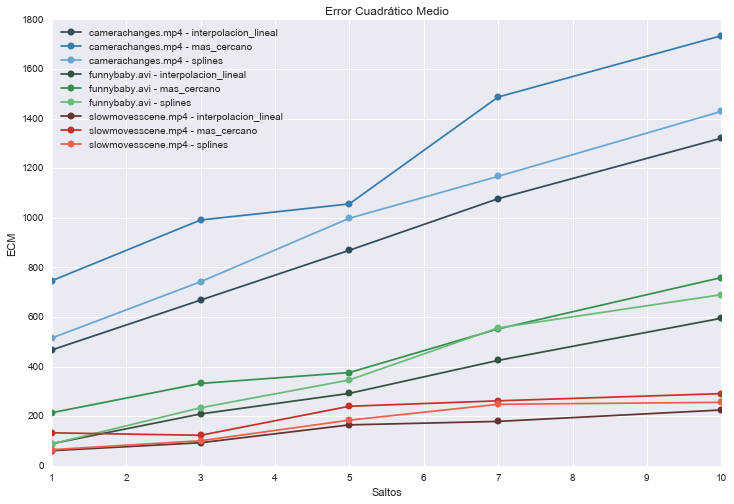
\includegraphics[width=.95\textwidth]{graficos/ecm.png}
\end{figure}

\vspace{-2em}
\begin{tiny}Este gr\'afico puede ser dificil de interpretar en blanco y negro\end{tiny}
\vspace{2em}

Este gr\'afico refuerza la hip\'otesis de que \textit{camerachanges.avi}, que tiene
muchos cambios de c\'amara, lo que hace que sea dificil predecir el valor de dos
pixeles cuando se pone en c\'amara lenta, tiene obviamente el mayor error. Por
otro lado, \textit{funnybaby.avi} y \textit{slowmoviescene.mp4} empiezan con un
\textbf{ECM} similar ya que ninguno de los dos tiene cambios bruscos, pero
cuando la cantidad de saltos aumenta el primer video empieza a tener un error
mucho mayor, ya que los cambios en el video dependientes del movimiento de la
cabeza del beb\'e \footnote{este es un beb\'e especialmente cabez\'on en comparaci\'on al
tama\~no del video} son mucho m\'as bruscos que los del video anterior.

Para comparar los m\'etodos, podemos ver el gr\'afico anterior y uno que tenga
solamente los valores para \textit{funnybaby.avi}

\begin{figure}[H]
\centering
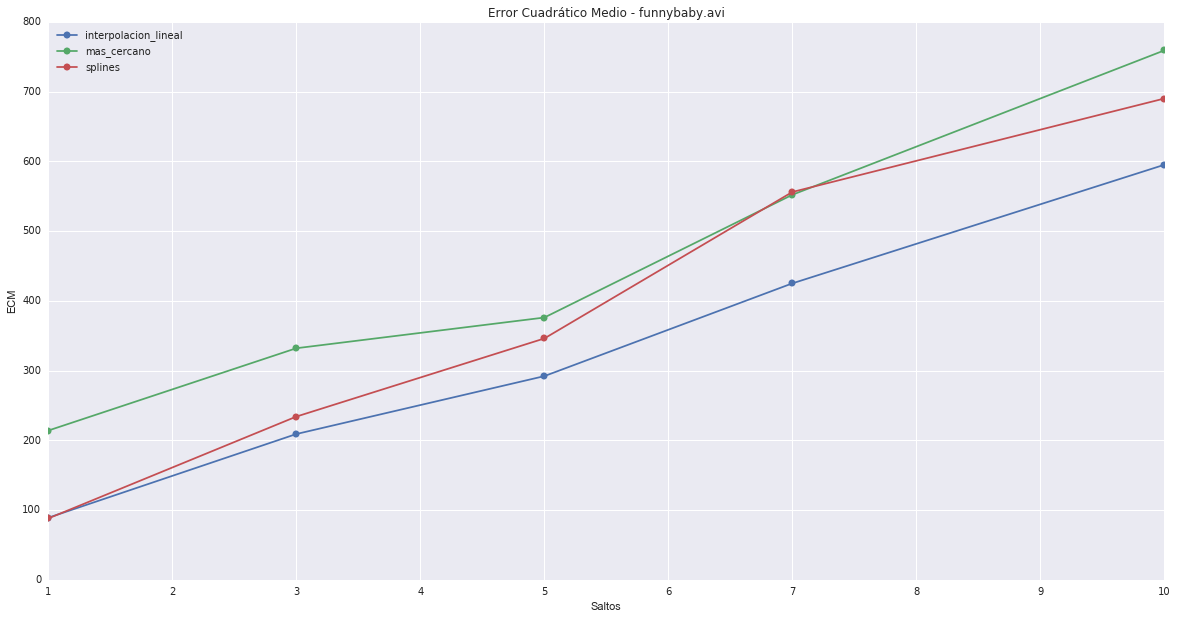
\includegraphics[width=.95\textwidth]{graficos/ecm_funnybaby.png}
\end{figure}

Como podemos ver, para nuestra sorpresa, en todos los videos el m\'etodo de \textbf{interpolaci\'on
lineal} es el que genera menores errores, inclusive menos que el de splines. Esto contradice nuestras
suposiciones de que splines, dada su complejidad extra para la generaci\'on de los frames, tendr\'ia 
un error inferior al de interpolaci\'on lineal.

El an\'alisis por \textbf{PSNR} da un resultado similar al de \textbf{ECM}, ya
que los dos m\'etodos est\'an inversamente relacionados. Sin embargo, se nota
con m\'as claridad que cuando hay pocos saltos el resultado puede ser altamente
diferente.

\begin{figure}[H]
\centering
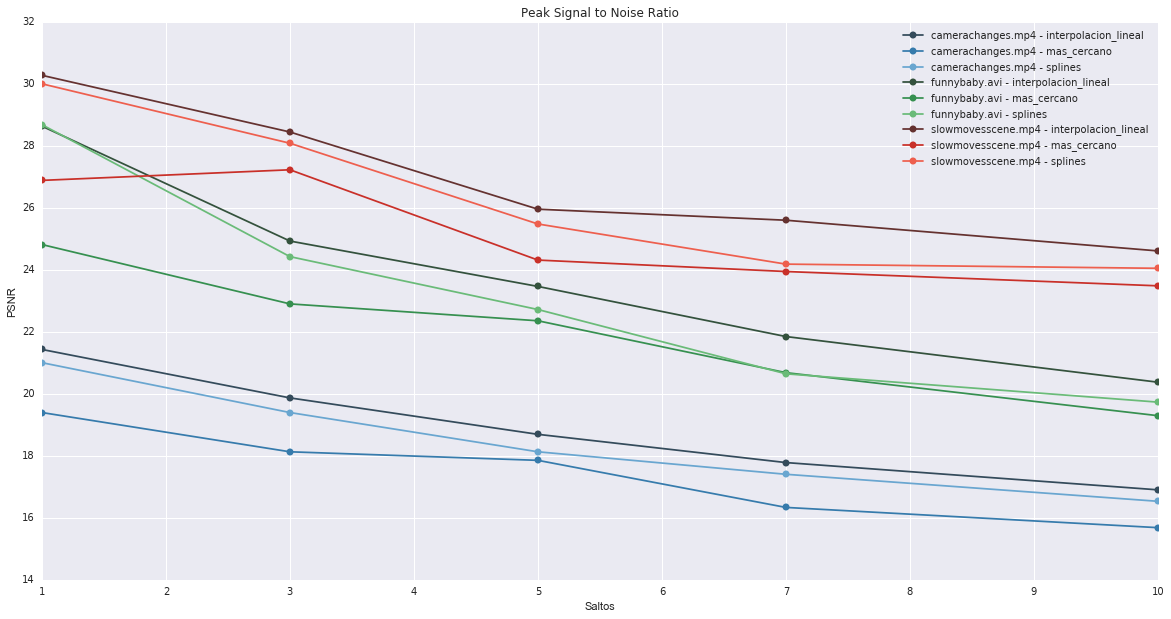
\includegraphics[width=.95\textwidth]{graficos/psnr.png}
\end{figure}
\vspace{-2em}
\begin{tiny}Este gr\'afico puede ser dificil de interpretar en blanco y negro\end{tiny}
\vspace{2em}

\subsubsection{An\'alisis de los m\'etodos frame por frame}

Como el calculo de \textbf{ECM}, que hasta ahora solo estamos promediando, se
hace por separado en cada frame, podemos hacer un an\'alisis por separado del
error medio en cada frame de algunos videos para poder encontrar cuanto cambiaba
este valor dependiendo de como se muevan, y si hay alg\'un m\'etodo que sea
preferible en alg\'un caso en particular.

Hicimos varias instancias de prueba similar a la del experimento anterior donde
habiendo un salto de \(2\) frames por cada frame del video original, ya que nos
parece una buena aproximaci\'on al caso real de alentizaci\'on de videos, y
calculamos el \textbf{ECM} entre cada uno de los frames generados y el frame
real.

\begin{figure}[H]
\centering
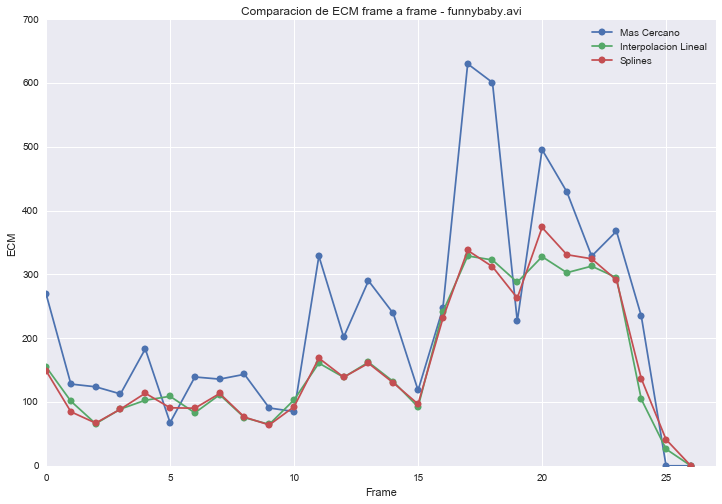
\includegraphics[width=.95\textwidth]{graficos/ecm_frame_funnybaby.png}
\end{figure}

Como \textit{funnybaby.avi} no tiene saltos ni ning\'un tipo de anormalidad en
todo el video, podemos ver que el \textbf{ECM} queda en el mismo orden de
magnitud por todo el an\'alisis. Sin embargo, podemos ver como este valor
aumenta considerablemente cuando el beb\'e del video hace una acci\'on que
cambia la mayor parte de los frames del video, como sacar la lengua o mover la
cabeza.

Al igual que en el an\'alisis del \textbf{ECM} promedio en el punto anterior,
con esta cantidad de saltos el valor de procesar el video con interpolaci\'on
lineal es similar a la de procesarlo con splines. Sin embargo, en este gr\'afico
tambi\'en se puede ver que aunque la diferencia entre el m\'etodo del m\'as
cercano con estos dos es similar cuando no hay muchos cambios, el error se
dispara cuando hay grandes cambios en la c\'amara.

Algo m\'as contundente pasa en el an\'alisis de otro video,
\textit{slowmovesscene.mp4}:

\begin{figure}[H]
\centering
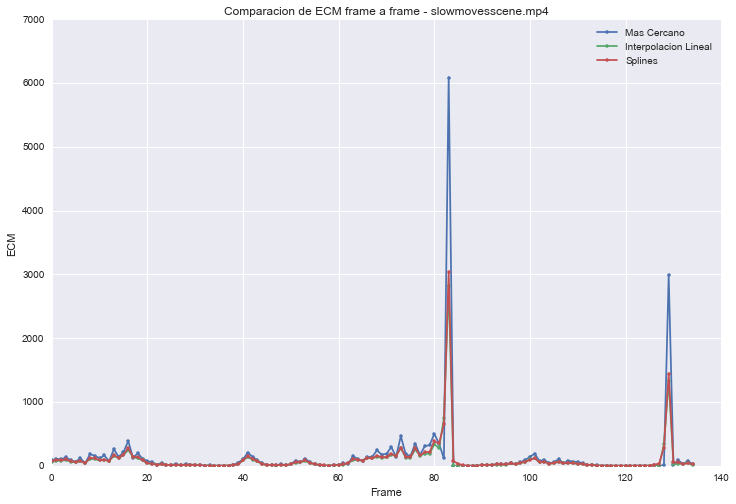
\includegraphics[width=.95\textwidth]{graficos/ecm_frame_slowmovescene.png}
\end{figure}

Este video tiene dos cambios de c\'amara importantes, y podemos ver que el
promedio del \textbf{ECM} se ve realmente afectado por los dos picos producidos
por estos cambios.

Como la distribuci\'on de los errores puede ser completamente diferente dentro y
fiera del pico, analizamos los dos casos por separado.

\begin{figure}[H]
\centering
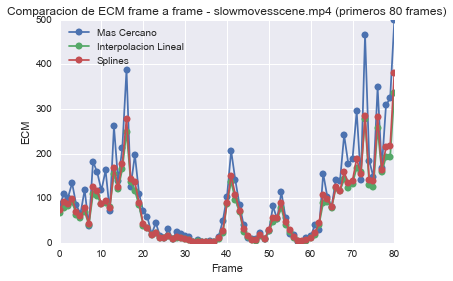
\includegraphics[width=.49\textwidth]{graficos/ecm_frame_slowmovescene_0_80.png}
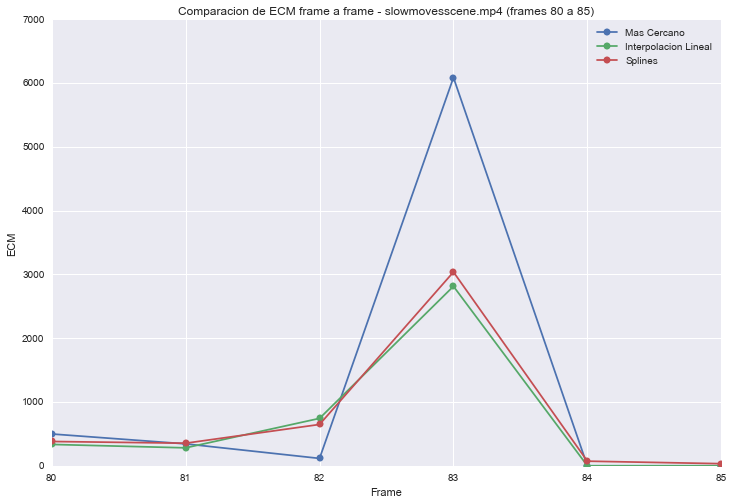
\includegraphics[width=.49\textwidth]{graficos/ecm_frame_slowmovescene_80_85.png}
\end{figure}

Podemos ver que en el gr\'afico que no incluye los picos tiene una
distribuci\'on similar a la de \textit{funnybaby.avi}, donde el m\'etodo de los
splines y el de interpolaci\'on lineal tienen resultados similares y el de
vecinos m\'as cercanos es considerablemente peor.

Sin embargo, haciendo zoom al pico m\'as grande, que pasa cuando la c\'amara
apunta al cielo, podemos varios patrones interesantes. Por ejemplo, el m\'etodo del
vecino m\'as cercano es el mejor por un solo frame cuando el video pasa por dos
frames seguidos en la misma imagen, ya que interpolaci\'on lineal y splines
intentan ser inteligentes y buscar un frame intermedio, mientras que el del
vecino m\'as cercano simplemente lo copia. Tambi\'en se puede ver que cuando se
hace el cambio de c\'amara, donde ninguno de los algoritmos puede predecir bien
cual va a ser el frame siguiente, el m\'etodo del vecino m\'as cercano es
considerablemente peor que los otros dos, y el de interpolaci\'on lineal es un
poco mejor al de splines.

\subsection{An\'alisis de la velocidad de los algoritmos}

\subsubsection{Comparaci\'on entre m\'etodos}

Todos los m\'etodos que usamos en la c\'amara lenta se aplican individualmente a
cada pixel, por lo tanto la complejidad temporal de los m\'etodos debe ser de la
forma $ \mathbb{O}(h \cdot w \cdot f^{(m)}(c_1)) $, con $h$ y $w$ alto y ancho del
video, respectivamente, $c_1$ la cantidad de frames del video final, y $f^{(m)}$
alguna funci\'on que depende del m\'etodo.

Como adem\'as ninguno de los tiempos de corrida de los m\'etodos cambia
dependiendo del valor de los pixeles \footnote{descontando el tiempo del
condicional cuando se pasa del rango de pixeles, que deber\'ia ser negligible},
una buena manera de medir la eficiencia de los m\'etodos es aplicandolos al
mismo video con diferente salto $s$ (ya que, para un $c_0$ fijo, tiene una
correlaci\'on lineal con $c_1$). Para este caso decidimos usar
\textit{baby.avi}.

Por cada m\'etodo, medimos la eficiencia de ese m\'etodo tomando el tiempo que
tarda en aplicar la c\'amara lenta a \textit{baby.avi} con diferentes 

\begin{figure}[H]
\centering
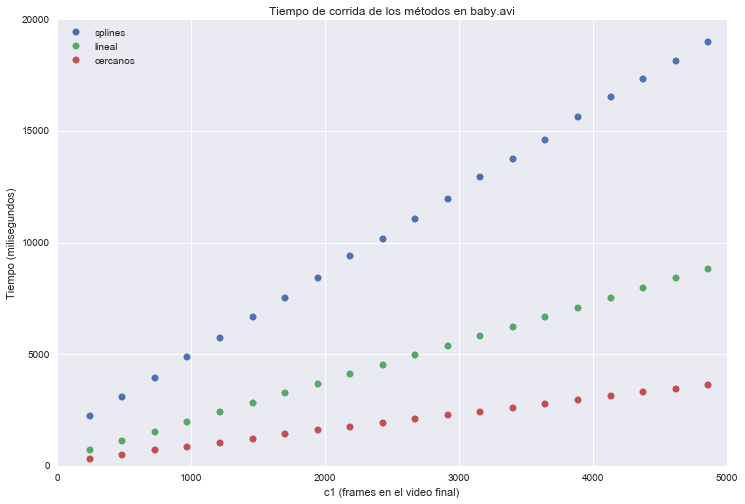
\includegraphics[width=.95\textwidth]{graficos/tiempo_baby.png}
\end{figure}

El gr\'afico da resultados previsibles: el tiempo de corrida del m\'etodo de los
splines es mayor que el de la interpolaci\'on lineal, que es mayor al de los
vecinos m\'as cercanos. Esto se debe a que, como explicado en el desarrollo,
el m\'etodo de los vecinos m\'as cercanos simplemente copia un valor de un
frame a otro y el de interpolaci\'on lineal hace una cuenta simple en punto
flotante, mientras que el de splines resuelve un sistema de $c_1$ ecuaciones.

Otra conclusi\'on que se puede sacar de este gr\'afico es que los tres m\'etodos
tiene complejidad temporal lineal. La raz\'on de esto es trivial en el caso de los
vecinos m\'as cercanos y el de la interpolaci\'on lineal, mientras que en el
caso de los splines nos aprovechamos que la matriz del sistema a resolver es
banda, lo que nos permite resolverlo en complejidad $\mathbb{O}(c_1)$ en vez de
la usual $\mathbb{O}(c_1^3)$.

\subsubsection{Reset en el m\'etodo de los splines}

Otro par\'ametro que puede tomar el \'ultimo m\'etodo, como est\'a explicado en
el desarrollo, es $r$, el ``reset'' del algoritmo. Esto indica que, en vez de
crear un sistema de ecuaciones para todos los puntos temporales en cada pixel,
va a crear sistemas de ecuaciones de tama\~no $r$ \footnote{posiblemente el
\'ultimo sea un poco m\'as grande}, y resolver cada sistema por separado.
Seg\'un nuestra hipotesis, esto deber\'ia resultar en un m\'etodo m\'as r\'apido
pero menos efectivo.

Para probarlo, dado que para probarlo eficientemente debemos hacerlo en videos
con un alto $c_1$, aprovechamos la propiedad de que el algoritmo funciona en
cada pixel por separado y creamos un video de tama\~no $1 \times 1$, con $c_0 =
100000$. De esta manera, podemos hacer las mismas pruebas m\'as r\'apido.

\begin{figure}[H]
\centering
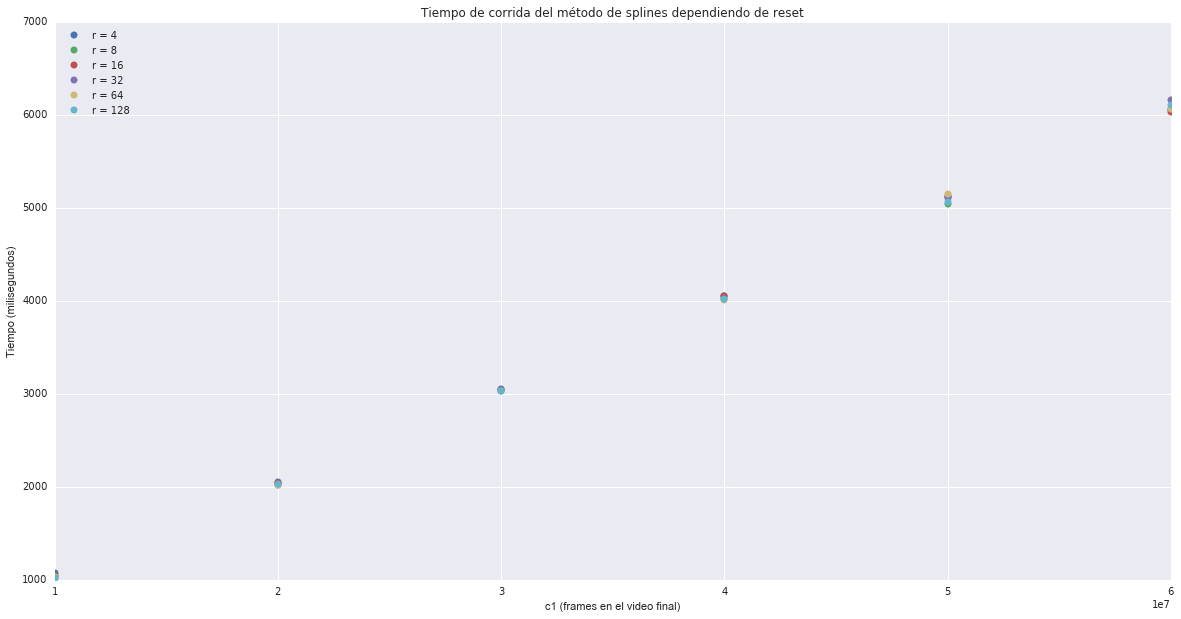
\includegraphics[width=.95\textwidth]{graficos/tiempo_reset.png}
\end{figure}

Por los resultados de los tiempos de la corrida podemos ver que nuestra
hip\'otesis es falsa. Al parecer, el algoritmo lineal para resolver el sistema
de ecuaciones con la matriz banda es lo suficientemente eficiente como para que
las ganancias de trabajar con matrices m\'as chicas sean despreciables cuando se
les suma el costo de preparar y juntar las soluciones.

Por otro lado, analizando el \textbf{ECM} de estas instancias, podemos ver que
el resultado es peor que en una corrida del algoritmo de Splines sin usar reset,
y cuanto m\'as seguido se haga el reset mayor va a ser el error.

\begin{figure}[H]
\centering
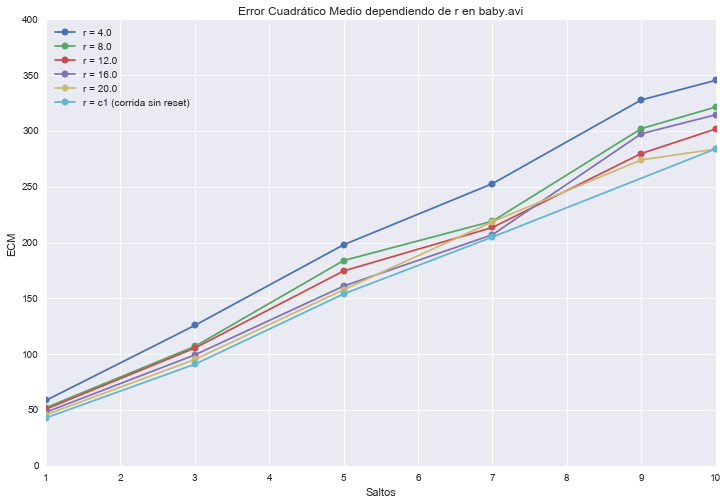
\includegraphics[width=.95\textwidth]{graficos/ecm_reset.png}
\end{figure}
